\documentclass[ignorenonframetext,]{beamer}
\setbeamertemplate{caption}[numbered]
\setbeamertemplate{caption label separator}{: }
\setbeamercolor{caption name}{fg=normal text.fg}
\beamertemplatenavigationsymbolsempty
\usepackage{lmodern}
\usepackage{amssymb,amsmath}
\usepackage{ifxetex,ifluatex}
\usepackage{fixltx2e} % provides \textsubscript
\ifnum 0\ifxetex 1\fi\ifluatex 1\fi=0 % if pdftex
\usepackage[T1]{fontenc}
\usepackage[utf8]{inputenc}
\else % if luatex or xelatex
\ifxetex
\usepackage{mathspec}
\else
\usepackage{fontspec}
\fi
\defaultfontfeatures{Ligatures=TeX,Scale=MatchLowercase}
\fi
% use upquote if available, for straight quotes in verbatim environments
\IfFileExists{upquote.sty}{\usepackage{upquote}}{}
% use microtype if available
\IfFileExists{microtype.sty}{%
\usepackage{microtype}
\UseMicrotypeSet[protrusion]{basicmath} % disable protrusion for tt fonts
}{}
\newif\ifbibliography

% Prevent slide breaks in the middle of a paragraph:
\widowpenalties 1 10000
\raggedbottom

\AtBeginPart{
\let\insertpartnumber\relax
\let\partname\relax
\frame{\partpage}
}
\AtBeginSection{
\ifbibliography
\else
\let\insertsectionnumber\relax
\let\sectionname\relax
\frame{\sectionpage}
\fi
}
\AtBeginSubsection{
\let\insertsubsectionnumber\relax
\let\subsectionname\relax
\frame{\subsectionpage}
}

\setlength{\parindent}{0pt}
\setlength{\parskip}{6pt plus 2pt minus 1pt}
\setlength{\emergencystretch}{3em}  % prevent overfull lines
\providecommand{\tightlist}{%
\setlength{\itemsep}{0pt}\setlength{\parskip}{0pt}}
\setcounter{secnumdepth}{0}
\usepackage{graphicx}

\title{Machine Learning and Deep Learning with R}
\author{Poo Kuan Hoong}
\date{February 15, 2017}

\begin{document}
\frame{\titlepage}

\begin{frame}{Deep Learning so far\ldots{}}

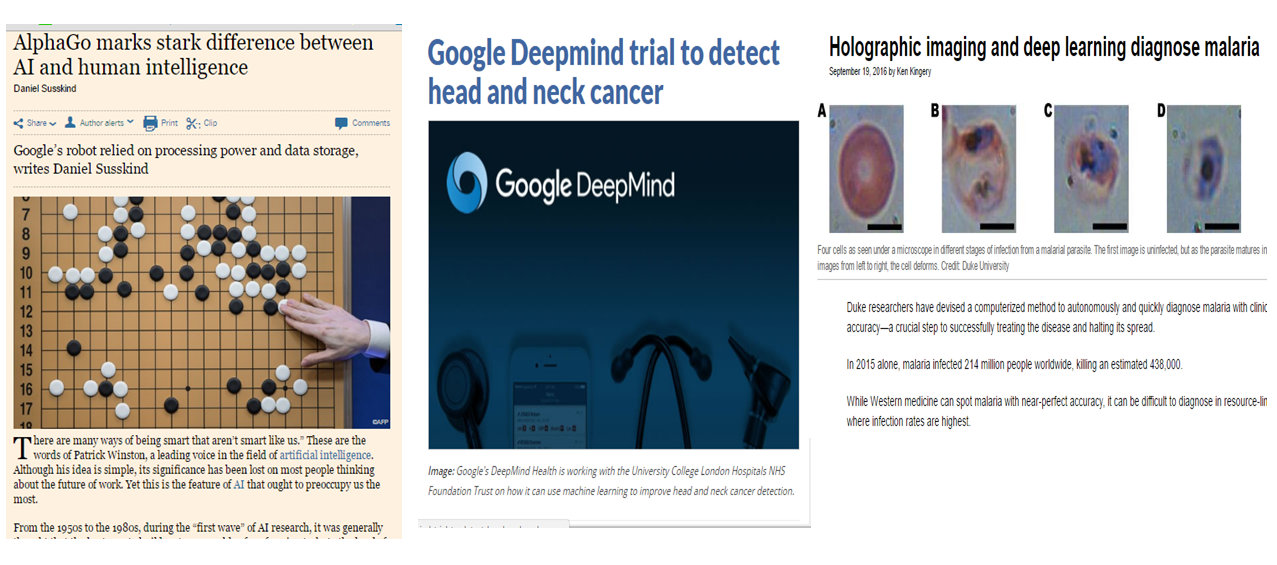
\includegraphics[width=300px]{images/deep_learning}

\end{frame}

\begin{frame}{Introduction}

\begin{itemize}
\tightlist
\item
  In the past 10 years, machine learning and Artificial Intelligence
  (AI) have shown tremendous progress
\item
  The recent success can be attributed to:

  \begin{itemize}
  \tightlist
  \item
    Explosion of data
  \item
    Cheap computing cost - CPUs and GPUs
  \item
    Improvement of machine learning models
  \end{itemize}
\item
  Much of the current excitement concerns a subfield of it called ``deep
  learning''.
\end{itemize}

\end{frame}

\begin{frame}{Human Brain}

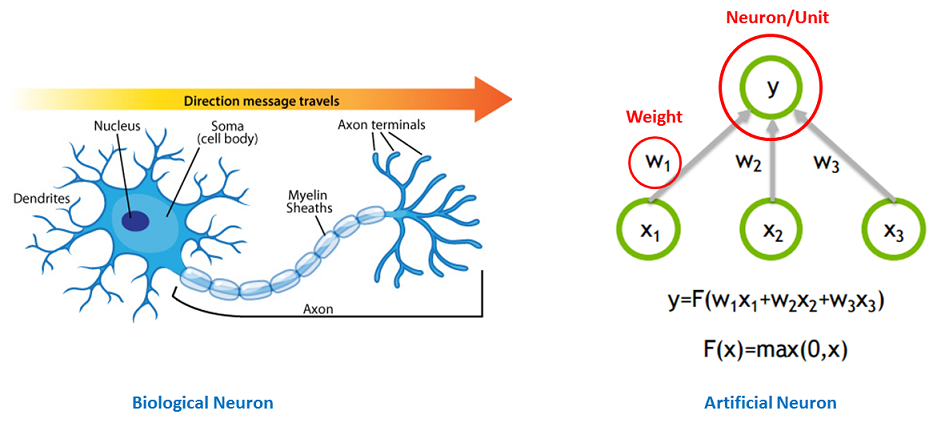
\includegraphics[width=300px]{images/brain}

\end{frame}

\begin{frame}{Neural Networks}

\begin{itemize}
\tightlist
\item
  Deep Learning is primarily about neural networks, where a network is
  an interconnected web of nodes and edges.
\item
  Neural nets were designed to perform complex tasks, such as the task
  of placing objects into categories based on a few attributes.
\item
  Neural nets are highly structured networks, and have three kinds of
  layers - an input, an output, and so called hidden layers, which refer
  to any layers between the input and the output layers.
\item
  Each node (also called a neuron) in the hidden and output layers has a
  classifier.
\end{itemize}

\end{frame}

\begin{frame}{Neural Network Layers}

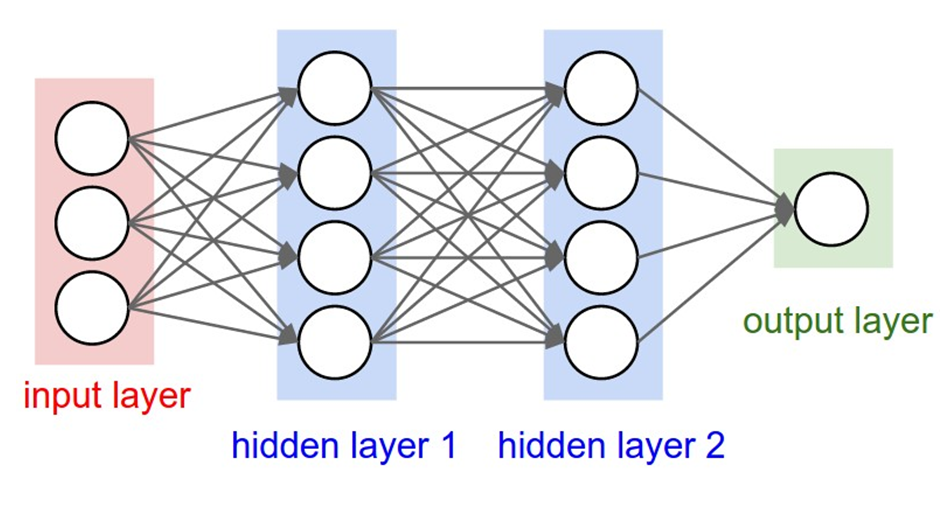
\includegraphics[width=300px]{images/neural_networks}

\end{frame}

\begin{frame}{Deep Learning}

\begin{itemize}
\tightlist
\item
  Deep learning refers to artificial neural networks that are composed
  of many layers.
\item
  It's a growing trend in Machine Learning due to some favorable results
  in applications where the target function is very complex and the
  datasets are large.
\end{itemize}

\end{frame}

\begin{frame}{Deep Learning: Benefits}

\begin{itemize}
\tightlist
\item
  Robust

  \begin{itemize}
  \tightlist
  \item
    No need to design the features ahead of time - features are
    automatically learned to be optimal for the task at hand
  \item
    Robustness to natural variations in the data is automatically
    learned
  \end{itemize}
\item
  Generalizable

  \begin{itemize}
  \tightlist
  \item
    The same neural net approach can be used for many different
    applications and data types
  \end{itemize}
\item
  Scalable

  \begin{itemize}
  \tightlist
  \item
    Performance improves with more data, method is massively
    parallelizable
  \end{itemize}
\end{itemize}

\end{frame}

\begin{frame}{Deep Learning: Weaknesses}

\begin{itemize}
\tightlist
\item
  Deep Learning \textbf{requires a large dataset}, hence long training
  period.
\item
  In term of cost, Machine Learning methods like SVMs and other tree
  ensembles are very easily deployed even by relative machine learning
  novices and can usually get you reasonably good results.
\item
  Deep learning methods \textbf{tend to learn everything}. It's better
  to encode prior knowledge about structure of images (or audio or
  text).
\item
  The learned features are often \textbf{difficult to understand}. Many
  vision features are also not really human-understandable (e.g,
  concatenations/combinations of different features).
\item
  Requires \textbf{a good understanding of how to model} multiple
  modalities with traditional tools.
\end{itemize}

\end{frame}

\begin{frame}{Deep Learning: Applications}

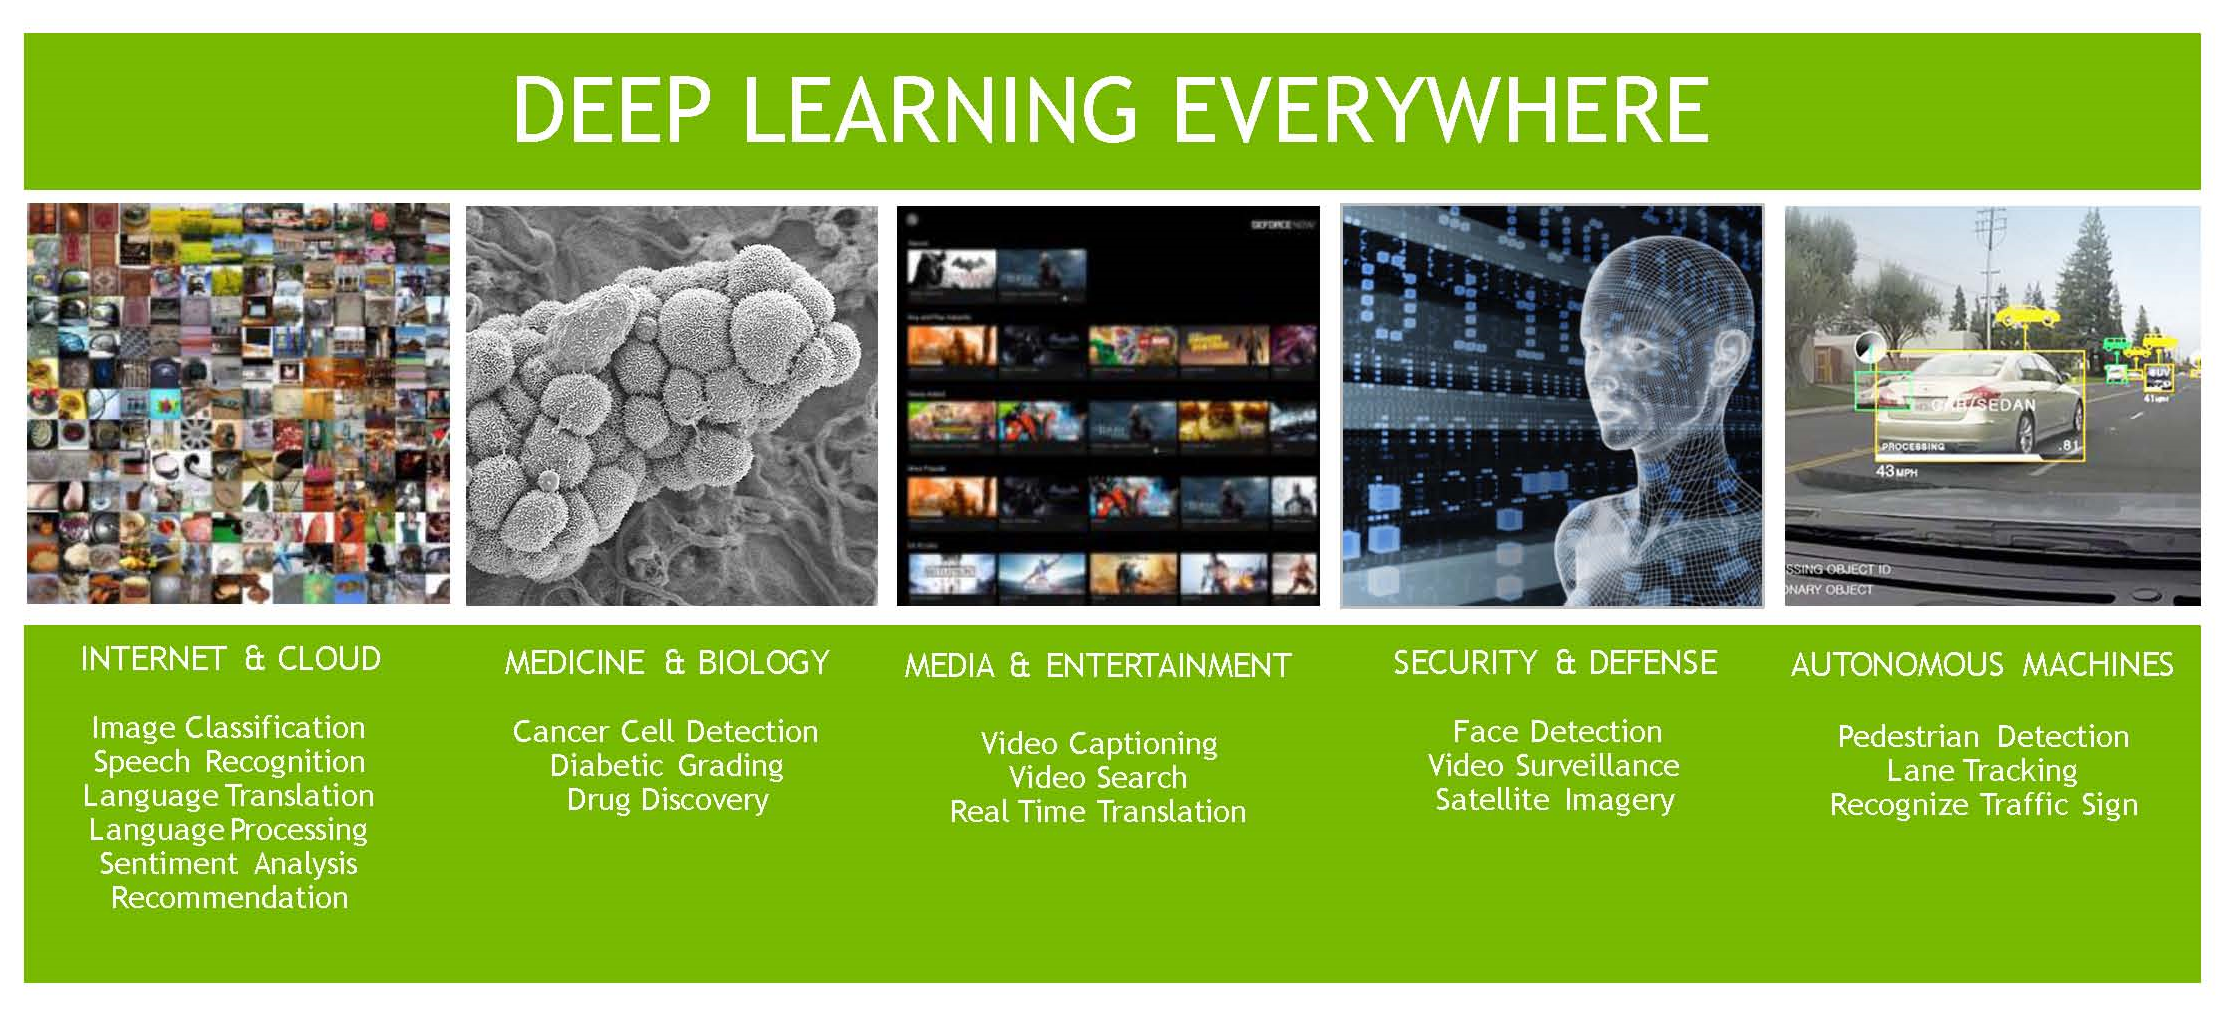
\includegraphics[width=300px]{images/deep_learning_applications}

\end{frame}

\begin{frame}{Deep Learning: R Libraries}

\begin{itemize}
\tightlist
\item
  \href{http://mxnet.io/api/r/index.html}{MXNet}: The R interface to the
  MXNet deep learning library.
\item
  \href{https://github.com/maddin79/darch}{darch}: An R package for deep
  architectures and restricted Boltzmann machines.
\item
  \href{https://mran.microsoft.com/package/deepnet/}{deepnet}: An R
  package implementing feed-forward neural networks, restricted
  Boltzmann machines, deep belief networks, and stacked autoencoders.
\item
  \href{https://github.com/h2oai/h2o-3}{h2o}: The R interface to the H2O
  deep-learning framework.
\end{itemize}

\end{frame}

\begin{frame}{MXNet}

\begin{center}


\includegraphics[width=70px]{images/mxnet} 
\end{center}

\begin{itemize}
\tightlist
\item
  \textbf{Founded by:} Uni. Washington \& Carnegie Mellon Uni
  (\textasciitilde{}1.5 years old)
\item
  \textbf{Supports most OS:} Runs on Amazon Linux, Ubuntu/Debian, OS X,
  and Windows OS
\item
  \textbf{State of the art model support:} Flexible and efficient GPU
  computing and state-of-art deep learning i.e.~CNN, LSTM to R.
\item
  \textbf{Ultra Scalable:} Seamless tensor/matrix computation with
  multiple GPUs in R.
\item
  \textbf{Ease of USe:} Construct and customize the state-of-art deep
  learning models in R, and apply them to tasks, such as image
  classification and data science challenges
\item
  \textbf{Multi-language:} Supports the Python, R, Julia and Scala
  languages
\item
  \textbf{Ecosystem:} Vibrant community from Academia and Industry
\end{itemize}

\end{frame}

\begin{frame}[fragile]{MXNet Architecture}

\begin{itemize}
\tightlist
\item
  You can specify the \texttt{Context} of the function to be executed
  within. This usually includes whether the function should be run on a
  CPU or a GPU, and if you specify a GPU, which GPU to use.
\end{itemize}

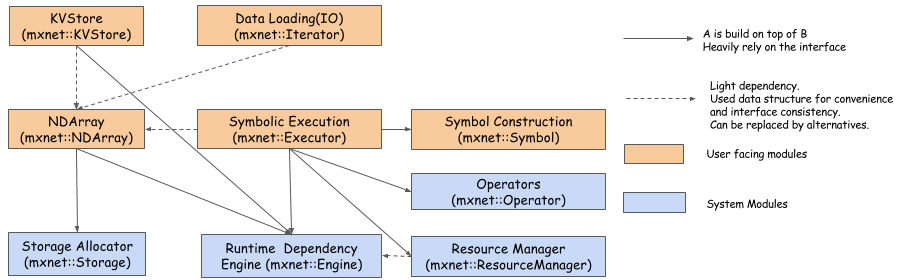
\includegraphics[width=300px]{images/mxnet_overview}

\end{frame}

\begin{frame}[fragile]{MXNet R Package}

\begin{itemize}
\tightlist
\item
  The R Package can be downloaded using the following commands:
\end{itemize}

\begin{verbatim}
install.packages("drat", repos="https://cran.rstudio.com")
drat:::addRepo("dmlc")
install.packages("mxnet")
\end{verbatim}

\end{frame}

\begin{frame}{Amazon \& MXNet for Deep Learning}

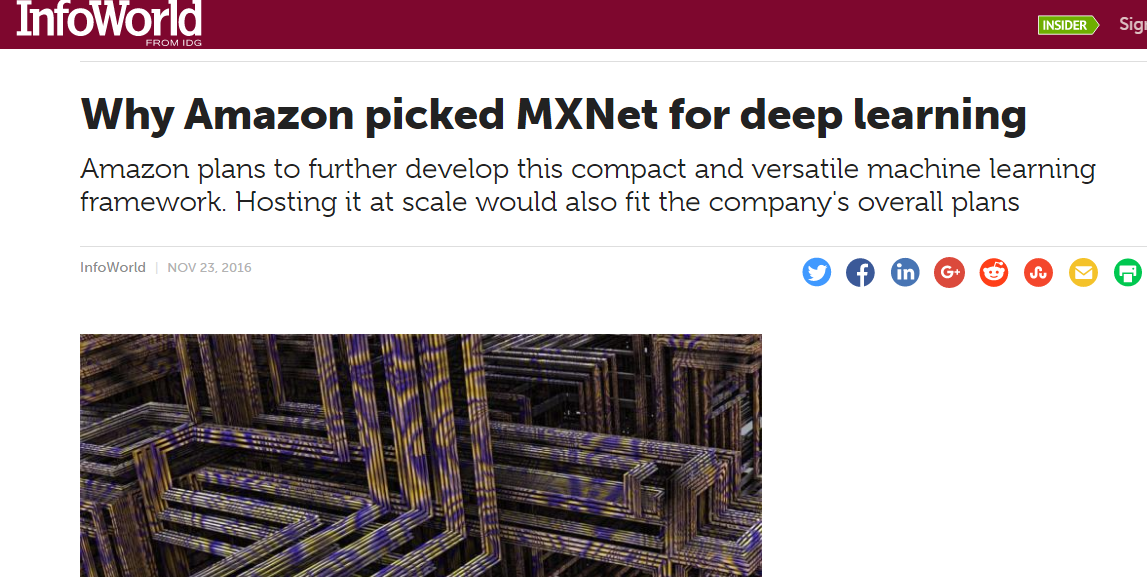
\includegraphics[width=300px]{images/amazon_mxnet}

\end{frame}

\begin{frame}{MNIST Handwritten Dataset}

\begin{itemize}
\tightlist
\item
  The MNIST database consists of handwritten digits.
\item
  The training set has 60,000 examples, and the test set has 10,000
  examples.
\item
  The MNIST database is a subset of a larger set available from NIST.
  The digits have been size-normalized and centered in a fixed-size
  image
\item
  For this demo, the Kaggle pre-processed training and testing dataset
  were used. The training dataset, (train.csv), has 42000 rows and 785
  columns.
\end{itemize}

\begin{center}

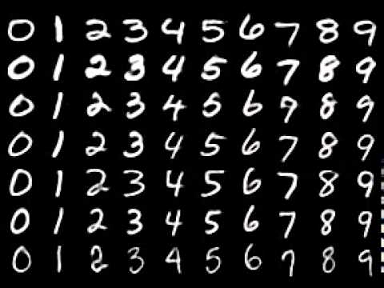
\includegraphics[width=100px]{images/mnist} 
\end{center}

\end{frame}

\begin{frame}{Demo}

\begin{itemize}
\tightlist
\item
  Sourcecode available here
  \url{https://github.com/kuanhoong/deeplearning-malaysia}
\end{itemize}

\end{frame}

\begin{frame}{Result}

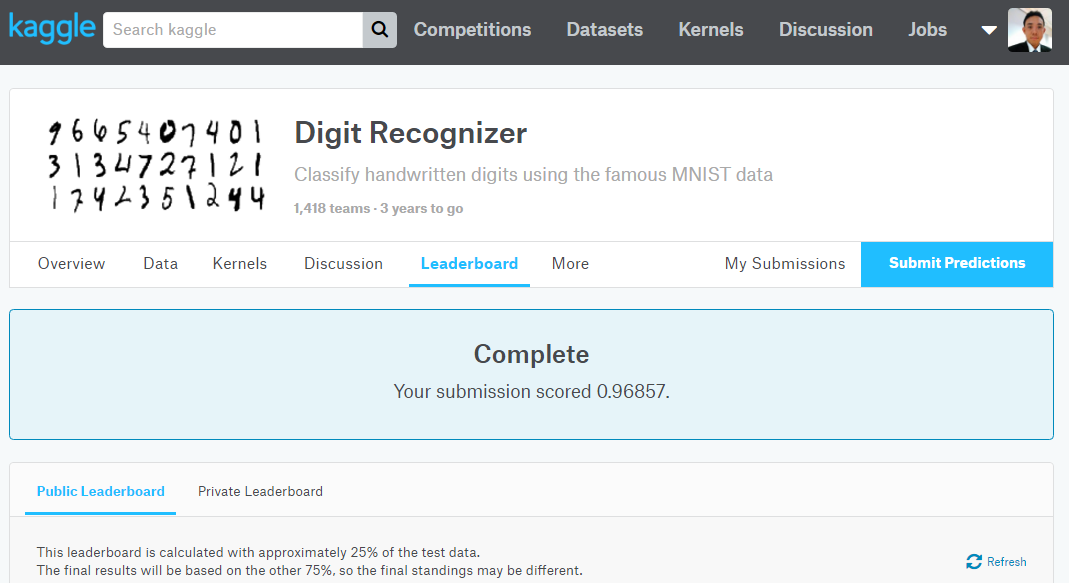
\includegraphics[width=300px]{images/mxnet-kaggle}

\end{frame}

\begin{frame}{Lastly\ldots{}}


\includegraphics[width=300px]{images/thankyou}

\end{frame}

\end{document}
